\documentclass[11pt,a4paper]{article}

\usepackage{kotex}
\usepackage{graphicx}
\usepackage{booktabs}
\usepackage{amsmath}
\usepackage{amssymb}
\usepackage{geometry}
\usepackage{hyperref}
\usepackage{xcolor}
\usepackage{caption}

\geometry{margin=25mm}
\hypersetup{
  colorlinks=true,
  linkcolor=blue,
  citecolor=blue,
  urlcolor=blue
}

\newcommand{\todo}[1]{\textcolor{red}{[TODO: #1]}}
\newcommand{\vis}{V}
\newcommand{\taugeo}{\tau}

\title{
약한 Starlink-like UEMR의 HERA-like delay/fringe 처리 후 잔류 구조와\\
다중 emitter delay-domain coherent-like amplification 검증
}
\author{
\todo{저자명}\\
\todo{소속}
}
\date{\today}

\begin{document}
\maketitle

\begin{abstract}
본 논문은 저궤도 위성에서 기인할 수 있는 Starlink-like unintended electromagnetic radiation (UEMR)이 HERA-like visibility 분석에서 어떻게 잔류하는지를 검증한다.
핵심 주장은 다음과 같다.
약한 Starlink-like UEMR은 raw visibility에서는 천체 foreground/background에 묻힐 수 있지만, weighted delay/fringe-rate 처리 이후 구조화된 interaction residual로 남을 수 있으며, 다중 emitter 조건에서는 delay-domain coherent-like amplification이 phase-randomized null ensemble의 95 percentile을 초과할 수 있다.

우리는 실제 HERA-like background visibility crop을 사용하고, TLE 기반 near-field geometry, HERA PolyBeam 기반 primary-beam response, Starlink-like literature-motivated spectrum, 그리고 Jones coherency 기반 polarization model을 결합하였다.
대표 mid-altitude window 세 개(w000--w002)에서 top-50 predicted apparent flux emitter subset을 사용했을 때 observed coherent-like amplification은 각각 6.93, 7.13, 7.16 dB였으며, 모든 경우에서 phase-randomized null의 95 percentile을 초과했다.
또한 unpolarized 및 Bassa et al.-motivated XX/YY anti-correlated polarization contrast sweep을 통해 polarization 가정이 EE/NN residual metric을 바꾸지만, coherent-like amplification claim 자체를 만들거나 제거하지는 않음을 확인했다.

본 결과는 proprietary Starlink waveform reconstruction이 아니며, D-terms, Faraday rotation, mutual coupling, 실제 Stokes U/V는 모델링하지 않는다.
따라서 본 논문의 클레임은 ``실제 Starlink waveform의 정확한 재현''이 아니라, TLE-constrained moving emitter contamination이 HERA-like delay/fringe pipeline에서 구조화된 residual 및 다중 emitter amplification risk를 만들 수 있다는 controlled-injection 검증이다.
\end{abstract}

\section{서론}

21 cm cosmology 관측은 foreground가 매우 강한 상황에서 약한 cosmological signal을 delay domain 및 fringe-rate domain에서 분리하려고 한다.
이때 문제는 단순히 radio-frequency interference (RFI)가 강한가의 여부가 아니라, pipeline 이후 남는 residual이 분석상 중요한 delay/fringe subspace에 구조적으로 남는가이다.
저궤도 통신 위성은 시간에 따라 빠르게 이동하고, baseline-dependent delay 및 fringe-rate를 가진다.
따라서 위성 UEMR contamination은 정지된 narrowband RFI와 달리 time-frequency visibility에서 이동체 geometry와 통신 texture를 동시에 가진다.

본 연구의 중심 질문은 다음과 같다.

\begin{quote}
약한 Starlink-like UEMR이 raw visibility에서는 background 아래에 있어도, HERA-like delay/fringe processing 이후 구조화된 interaction residual로 남고, 다중 emitter 조건에서 phase-randomized null을 초과하는 delay-domain coherent-like amplification을 만들 수 있는가?
\end{quote}

본 논문은 위 질문에 대해 controlled-injection 방식으로 답한다.
우리는 sky/background 자체를 내부 toy model로 만들지 않고, 외부 HERA-like UVH5-derived visibility crop을 background로 사용한다.
Starlink-like component만 TLE 기반 near-field geometry 및 literature-motivated spectrum으로 주입한다.
분석 product는 단순한 injected visibility가 아니라
\begin{equation}
  \vis_{\rm int}
  =
  {\cal P}(\vis_{\rm bg}+\vis_{\rm sat})
  -
  {\cal P}(\vis_{\rm bg})
\end{equation}
로 정의되는 interaction residual이다.
여기서 ${\cal P}$는 weighted delay high-pass 및 fringe-rate filtering chain을 뜻한다.

\subsection{본 논문의 클레임}

본 논문의 주장은 의도적으로 좁게 잡는다.
우리는 Starlink 위성의 실제 proprietary waveform을 복원하거나, 특정 관측 night에서 실제 Starlink event를 검출했다고 주장하지 않는다.
또한 본 논문은 HERA의 full calibration chain, redundant calibration, full Stokes calibration, direction-dependent leakage calibration을 재현하지 않는다.
대신 본 논문은 다음 controlled claim을 검증한다.

\begin{enumerate}
  \item TLE-constrained moving emitter는 baseline-dependent near-field delay 및 fringe-rate를 가지며, static narrowband RFI와 다른 residual morphology를 만든다.
  \item Raw visibility에서 background 아래에 있는 weak injected UEMR도 delay/fringe processing 이후 interaction residual로 구조화되어 남을 수 있다.
  \item 여러 emitter가 같은 delay bin에 일정 시간 이상 overlap하면, complex sum의 delay-excess power가 incoherent sum보다 커질 수 있다.
  \item 이 coherent-like amplification은 random phasor addition만으로 설명되는지 확인하기 위해 phase-randomized null ensemble과 비교해야 한다.
  \item Bassa et al.-style XX/YY anti-correlation은 full-Stokes measurement가 아니라 parameterized Stokes-Q contrast로 취급해야 하며, polarization sensitivity로 claim의 안정성을 확인해야 한다.
\end{enumerate}

위 다섯 항목이 본문 실험 A--E의 구조를 결정한다.
따라서 본 논문에서 중요한 것은 새로운 toy model을 계속 추가하는 것이 아니라, 각 claim을 reviewer가 반박하기 어려운 metric으로 닫는 것이다.
예를 들어 ``복소합을 하면 원래 커지는 것 아닌가''라는 반박은 phase-randomized null로 닫고, ``왜 top-50인가''라는 반박은 top-N sensitivity로 닫는다.
``전체 background보다 약한데 왜 중요한가''라는 반박은 global power가 아니라 local/EoR-window delay-bin residual budget으로 답한다.

\subsection{비클레임과 해석 범위}

다음 사항은 본 논문의 범위 밖이다.

\begin{itemize}
  \item 실제 Starlink telemetry, modulation, beam steering schedule, proprietary waveform의 reconstruction.
  \item 특정 HERA observing night에서 실제 satellite contamination을 blind detection했다는 주장.
  \item full direction-dependent calibration이나 redundant calibration residual의 완전한 propagation.
  \item 실제 satellite Stokes $U,V$ 또는 circular polarization의 측정.
  \item antenna D-terms, mutual coupling, ionospheric Faraday rotation의 full Jones propagation.
\end{itemize}

이 비클레임을 명확히 하는 이유는 본 연구가 ``현실을 완전히 모사한 simulation''이 아니라, HERA-like delay/fringe processing blind spot을 검증하는 controlled experiment이기 때문이다.
즉 우리는 주어진 background visibility 위에 physically constrained moving emitter를 올리고, pipeline output의 residual metric을 비교한다.
이 접근은 real-data detection paper보다 좁지만, 특정 mechanism을 isolation하여 검증하기에는 더 적합하다.

\section{관련 연구와 배경}

\subsection{LEO satellite UEMR와 low-frequency radio astronomy}

저궤도 통신 위성 constellation의 증가는 low-frequency radio astronomy에 새로운 systematic risk를 만든다.
특히 Starlink-like 위성은 의도된 downlink band 밖에서도 unintended electromagnetic radiation을 만들 수 있으며, 이는 LOFAR 등 low-frequency array에서 보고된 바 있다.
\todo{Di Vruno et al. 2023, Bassa et al. 2024의 구체적 frequency, flux density, instrument 설정을 문헌 표로 정리}

중요한 점은 UEMR이 단순히 ``강한 RFI''인가가 아니다.
21 cm cosmology에서는 foreground가 이미 cosmological signal보다 훨씬 크기 때문에, contamination risk는 total power가 아니라 spectral smoothness, delay-domain leakage, calibration coupling, residual subspace overlap에 의해 결정된다.
따라서 약한 moving transmitter라도 delay/fringe filtering 이후 특정 분석 영역에 구조화된 residual을 만들면 문제가 될 수 있다.

\subsection{Delay-spectrum 관점}

Interferometric visibility에서 frequency direction Fourier transform은 delay domain을 만든다.
짧은 baseline의 smooth foreground는 주로 horizon delay 안쪽에 집중된다고 기대되며, 이 바깥 영역은 EoR window로 불린다.
물론 실제 instrument chromaticity, flagging, calibration error, beam sidelobe, finite bandwidth windowing은 foreground leakage를 만든다.
본 논문의 contamination metric은 이러한 delay-domain 관점에서 정의된다.
우리는 residual이 total processed background power를 지배하는지를 묻지 않고, delay-excess region에서 background 대비 얼마나 올라오는지를 측정한다.

\subsection{Moving emitter와 fringe-rate}

LEO satellite는 시간에 따라 apparent position, range, delay, fringe-rate가 빠르게 변한다.
이 점은 static RFI와 다르다.
특히 baseline-dependent phase
\[
  \exp[-2\pi i\nu\tau_{ij}(t)]
\]
가 시간에 따라 변하므로, emitter의 contamination은 time-frequency plane에서 deterministic but moving structure를 가진다.
이 구조는 finite integration, finite channel width, fringe-rate filtering과 상호작용한다.
따라서 raw waterfall에서 눈에 잘 보이지 않던 component가 processing 후 residual pattern으로 남을 수 있다.

\subsection{Polarization issue}

Bassa et al.에서 보고된 XX/YY anti-correlation은 본 연구에서 중요한 동기이다.
그러나 이 관측을 곧바로 satellite emission의 full Stokes measurement로 해석하는 것은 과도하다.
따라서 우리는 anti-correlation을 Stokes-Q contrast parameterization으로만 사용한다.
이 모델은 EE/NN sensitivity를 확인하기 위한 perturbation model이며, 실제 $U,V$ 또는 D-term leakage를 설명하지 않는다.
이 보수적 포지셔닝은 Methods와 Limitation에 반복해서 명시한다.

\section{데이터와 실험 설정}

\subsection{Background visibility}

실험에는 HERA-like UVH5에서 추출한 단일 baseline crop을 사용하였다.
대표 baseline은 antenna pair $(0,5)$이며 baseline length는 약 73.04 m, orientation은 EW이다.
주파수 범위는 약 110--190 MHz이고, window crop은 1시간 단위로 분할하였다.
현재 본문 검증에는 w000, w001, w002 세 개의 1시간 window를 사용하였다.

원본 UVH5를 매번 전체 load하면 runtime timeout과 I/O 병목이 발생하므로, 분석은 1시간 NPZ chunk 단위로 수행하였다.
각 chunk는 동일한 antenna pair, 동일한 polarization product, 동일한 frequency crop을 가진다.
이 방식은 실험을 window 단위로 재시작할 수 있게 하며, 실패한 run이 전체 sweep을 망치지 않도록 한다.
또한 각 window가 끝날 때마다 summary CSV를 flush하여 timeout이나 I/O error가 발생해도 완료된 window의 metric은 보존된다.

현재 사용한 background chunk는 다음과 같다.

\begin{itemize}
  \item \texttt{background\_0\_5\_w000\_1h.npz}
  \item \texttt{background\_0\_5\_w001\_1h.npz}
  \item \texttt{background\_0\_5\_w002\_1h.npz}
\end{itemize}

각 chunk는 약 373 time samples와 656 frequency channels를 포함한다.
\todo{정확한 integration time, channel width, LST/JD range를 table에 추가}

\begin{table}[t]
\centering
\caption{대표 validation window의 emitter selection 요약. mid-altitude gate는 peak altitude 35--70 degree이다.}
\label{tab:window-summary}
\begin{tabular}{lrrrrr}
\toprule
Window & Visible total & Mid-alt count & Used emitters & Observed amp. [dB] & Null p95 [dB]\\
\midrule
w000 & 836  & 184 & 50 & 6.93 & 2.18\\
w001 & 889  & 243 & 50 & 7.13 & 2.03\\
w002 & 1071 & 318 & 50 & 7.16 & 2.02\\
\bottomrule
\end{tabular}
\end{table}

\subsection{Invalid sample mask}

Waterfall figure에서 background에 흰색 horizontal stripe가 나타났기 때문에 NaN/Inf/weight metadata를 확인하였다.
그 결과 해당 stripe는 plot clipping artifact나 zero-weight region이 아니라 raw background 자체의 NaN region이었다.

\begin{itemize}
  \item raw background NaN count: 243
  \item raw background Inf count: 0
  \item weights zero count: 0
  \item weights nonfinite count: 0
  \item NaN rows: 96, 146, 149
  \item NaN frequency range: 138.35--148.12 MHz
\end{itemize}

따라서 논문 figure에서는 invalid samples를 signal로 해석하지 않고 회색 mask overlay로 표시한다.

이 mask 처리는 중요한 sanity step이다.
만약 invalid samples가 흰색 high-amplitude stripe처럼 보이면, 독자는 이를 satellite residual이나 processing artifact로 오해할 수 있다.
그러나 metadata 확인 결과 weights는 모두 1이고 zero-weight region이 아니었다.
따라서 해당 region은 background product 자체의 missing/NaN sample이며, injection 또는 delay/fringe processing이 만든 구조가 아니다.
본문 figure에서는 이 영역을 회색으로 표시하고, quantitative metric 계산에서는 finite-value handling을 명확히 한다.
\todo{metric 계산에서 NaN이 weighted transform에서 0으로 대체되는 정확한 implementation detail을 appendix에 코드 수준으로 기술}

\subsection{Window selection}

초기 run에서는 peak altitude가 약 87 degree인 near-zenith pass가 선택되어, range minimum, beam maximum, smearing structure가 pass center에 과도하게 집중되었다.
이 경우 injection support가 중앙 horizontal burst처럼 보이며, representative main-text example로 부적합했다.
따라서 main controlled-injection set에서는 peak altitude gate를 도입하였다.
본문의 main validation은
\[
35^\circ \le h_{\rm peak} \le 70^\circ
\]
인 mid-altitude emitter만 사용한다.
이 선택은 zenith-crossing compression을 피하고, time direction에서 더 자연스러운 pass morphology를 얻기 위한 것이다.

이 gate는 satellite visibility 자체를 약하게 만들기 위한 것이 아니라, representative morphology를 확보하기 위한 quality control이다.
고도 gate에 따른 sensitivity는 아직 선택 실험으로 남아 있으며, Sec.~\ref{sec:future}에서 TODO로 표시한다.

\subsection{Reproducibility artifacts}

각 run은 다음 output artifact를 생성한다.

\begin{itemize}
  \item \texttt{tables/multi\_window\_summary.csv}: window-level metric.
  \item \texttt{tables/per\_satellite\_window\_summary.csv}: selected emitter별 peak altitude, range, realized amplitude, cap score.
  \item \texttt{tables/pairwise\_delay\_coherence.csv}: pairwise delay overlap 및 coherence metric.
  \item \texttt{tables/phase\_randomized\_null\_ratios.csv}: phase-randomized null trial별 amplification ratio.
  \item \texttt{figures/}: waterfall, null histogram, pairwise scatter, local budget bar plot.
  \item \texttt{config\_used.yaml}: run-specific resolved config.
\end{itemize}

원본 UVH5는 크기와 provenance 문제 때문에 repository에 포함하지 않는다.
대신 cropped NPZ, summary CSV, figure, config, code path를 통해 controlled experiment를 재현할 수 있게 한다.
\todo{최종 공개 repository에서는 raw data policy와 Zenodo/Dataverse 여부를 명시}

\section{Starlink-like UEMR injection model}

\subsection{Near-field geometry}

각 satellite emitter의 delay는 far-field 근사 $ \mathbf{b}\cdot \hat{\mathbf{s}}/c $가 아니라 antenna-to-satellite range difference로 계산하였다.
\begin{equation}
  \tau_{ij}(t)
  =
  \frac{
  \left|\mathbf{r}_{\rm sat}(t)-\mathbf{r}_{j}\right|
  -
  \left|\mathbf{r}_{\rm sat}(t)-\mathbf{r}_{i}\right|
  }{c}.
\end{equation}
이에 따른 complex visibility phase는
\begin{equation}
  \phi(t,\nu)=\exp[-2\pi i\nu\tau_{ij}(t)]
\end{equation}
로 적용하였다.
Finite integration 및 finite channel bandwidth에 따른 attenuation은 sinc 계열 smearing factor로 적용하였다.
\todo{smearing 식과 정확한 config parameter를 Methods appendix에 추가}

\subsection{Flux, range, beam, scheduler modulation}

Source amplitude는 reference flux density, range attenuation, primary-beam response, finite smearing, duty/scheduler modulation, 그리고 spectral template의 곱으로 구성하였다.
reference flux는 관측된 final visibility amplitude가 아니라, pre-beam, pre-smearing, reference-range scale parameter이다.
따라서 모든 run에서는 realized visibility amplitude 및 local residual metric을 별도로 보고한다.

Range attenuation은 기본적으로
\begin{equation}
  A_{\rm range}(t)=\left(\frac{r_{\rm ref}}{r(t)}\right)^2
\end{equation}
를 사용하였다.
Primary beam은 \texttt{hera\_sim}의 PolyBeam-like Fagnoni model을 사용하되, Chebyshev extrapolation으로 인한 unphysical excursion은 applied power response를 0--1로 clip하고 raw extrema는 metadata에 저장하였다.

이 beam clipping은 과학적 임의 조정이 아니라 sanity protection이다.
PolyBeam polynomial은 fitted domain 밖 또는 특정 numerical regime에서 unphysical large response를 만들 수 있다.
실제로 early validation에서 applied beam response가 $10^{16}$--$10^{20}$ 수준까지 커지는 satellite/window가 있었고, 이는 flux/range/beam unit mismatch처럼 보이는 catastrophic amplitude를 만들었다.
따라서 code는 다음 hard gate와 metadata를 사용한다.

\begin{itemize}
  \item applied beam power response는 0--1 범위로 clip한다.
  \item raw power min/max는 \texttt{beam\_meta}에 저장한다.
  \item applied \texttt{beam\_max}가 10을 넘거나 raw injected amplitude가 $10^6$ Jy를 넘으면 sanity failure로 처리한다.
\end{itemize}

이렇게 해야 reference flux parameter가 unphysical beam excursion 때문에 final result를 지배하는 상황을 방지할 수 있다.

\subsection{Amplitude sanity}

본 실험에서 \texttt{reference\_flux\_jy}는 observed contamination amplitude가 아니다.
이는 reference range에서 pre-beam, pre-smearing, pre-duty scale을 정하는 parameter이다.
실제 injected visibility amplitude는 range attenuation, beam response, finite smearing, scheduler duty, polarization projection을 모두 거친 뒤 결정된다.
따라서 각 run은 다음 sanity quantities를 기록한다.

\begin{itemize}
  \item \texttt{beam\_max}
  \item \texttt{range\_att\_max}
  \item \texttt{spectrum\_jy\_max}
  \item \texttt{raw\_starlink\_peak\_abs}
  \item \texttt{raw\_background\_peak\_abs}
\end{itemize}

논문에서는 reference flux와 realized visibility amplitude를 혼동하지 않는다.
예를 들어 100 Jy 또는 300 Jy scale parameter가 곧 관측 visibility에서 100 Jy contamination을 뜻하는 것은 아니다.
Methods text에서는 이를 ``pre-beam, pre-smearing reference-scale parameter''로 표현한다.

\subsection{Emitter cap selection}

다중 emitter window에서 모든 visible TLE object를 주입하면 계산량과 interpretation이 불필요하게 커지므로, 본문 실험에서는 top-N cap을 적용하였다.
cap 기준은 고정된 deterministic score로 정의한다.
\begin{equation}
  S_{\rm cap}
  =
  S_{\rm ref}
  \left(\frac{r_{\rm ref}}{r_{\rm peak}}\right)^2
  \sin^2(h_{\rm peak}),
\end{equation}
여기서 $h_{\rm peak}$는 window 내 peak altitude이다.
즉 main selection은 ``top 50 by predicted peak apparent flux''이다.
top-N sensitivity는 Sec.~\ref{sec:topn}에서 검증한다.

\subsection{Communication texture}

Starlink-like UEMR model은 완전한 proprietary waveform이 아니다.
대신 literature-motivated spectral structure와 scheduler-like time/frequency modulation을 사용한다.
이 선택은 두 가지 목적을 가진다.
첫째, 전체 band가 동시에 켜지는 toy stripe를 피한다.
둘째, moving transmitter contamination morphology가 subband/comb-like feature와 satellite delay track을 동시에 갖도록 한다.

현재 implementation은 다음 요소를 포함한다.
\begin{itemize}
  \item literature-motivated UEMR spectral template 또는 parameterized measured component.
  \item duty-cycle modulation.
  \item finite channel dilution for narrow sub-channel features.
  \item frequency-dependent spectral slope.
\end{itemize}

다만 이 texture는 실제 Starlink waveform reconstruction이 아니며, Methods와 Conclusion에서 이 제한을 명시한다.
\todo{최종본에서는 사용한 literature model parameter table을 추가}

\section{Polarization model}

Starlink UEMR의 실제 full-Stokes coherency는 공개적으로 확정되어 있지 않다.
따라서 본 논문은 Bassa et al.에서 보고된 XX/YY anti-correlation을 full Stokes measurement로 해석하지 않고, parameterized Stokes-Q contrast로 취급한다.

Source coherency matrix는 다음과 같이 둔다.
\begin{equation}
  C_{\rm src}
  =
  \begin{pmatrix}
  I + Q & U+iV\\
  U-iV & I-Q
  \end{pmatrix}.
\end{equation}
Unpolarized model에서는 $Q=U=V=0$이다.
Anti-correlated model에서는
\begin{equation}
  Q(t,\nu)
  =
  \eta\,I(t,\nu)\sin(2\pi t/T+\phi_0),
\end{equation}
로 parameterize하였다.
여기서 $\eta$는 contrast이다.

Antenna response는 diagonal Jones approximation을 사용한다.
\begin{equation}
  \vis_{ij}(t,\nu)
  =
  J_i(t,\nu)\,C_{\rm src}(t,\nu)\,J_j^\dagger(t,\nu).
\end{equation}
현재 구현은 D-terms, mutual coupling, ionospheric Faraday rotation, 실제 Stokes U/V를 포함하지 않는다.
이 제한은 본문과 conclusion에 명시한다.

\section{Pipeline 및 metric}

\subsection{Processing operator}

본 논문에서 ${\cal P}$는 full HERA calibration pipeline이 아니다.
${\cal P}$는 명시적으로 정의된 weighted delay/fringe-rate processing operator이다.
구체적으로는 frequency direction taper를 적용한 weighted delay transform, horizon-plus-buffer 안쪽 mode 제거 또는 high-pass selection, 그리고 선택적인 fringe-rate notch/filter로 구성된다.
Flagged 또는 non-finite visibility value는 median replacement하지 않고, weight를 통해 transform에 들어간다.
이 점은 중요하다.
왜냐하면 flag replacement나 interpolation은 satellite-like structure를 인위적으로 만들거나 지울 수 있기 때문이다.
본 실험에서는 missing/invalid sample을 signal로 해석하지 않고, figure에서는 mask로 표시한다.

Processing operator를 명시적으로 제한한 이유는 본 논문의 claim을 calibration residual 전체로 확장하지 않기 위해서이다.
Redundant calibration, sky model subtraction, gain solution error, cable reflection, cross-talk은 별도의 systematics이다.
본 논문은 그보다 좁게, moving emitter visibility가 delay/fringe filtering 이후 interaction residual로 남는지 확인한다.

\subsection{Interaction residual}

분석 product는 injected satellite visibility 자체가 아니라, processing 이후 background와 dirty visibility의 차이다.
\begin{equation}
  \vis_{\rm residual}
  =
  {\cal P}(\vis_{\rm background}+\vis_{\rm satellite})
  -
  {\cal P}(\vis_{\rm background}).
\end{equation}
이 정의는 weak contamination이 total processed background power를 지배하지 않더라도, delay/fringe processing 이후 structured residual로 남는지를 측정하기 위한 것이다.

\subsection{Coherent-like amplification}

다중 emitter visibility를
\begin{equation}
  \vis_{\rm sum}=\sum_k \vis_k
\end{equation}
로 두고, delay-excess power metric을 $P(\cdot)$라고 하면 observed amplification ratio는
\begin{equation}
  R_{\rm obs}
  =
  \frac{P(|\sum_k \vis_k|)}{\sum_k P(|\vis_k|)}
\end{equation}
로 정의한다.
복소합 자체가 random phasor addition으로도 커질 수 있다는 반박을 막기 위해, 각 emitter의 amplitude와 delay support는 유지하되 emitter별 complex phase를 randomize한 null ensemble을 만든다.
\begin{equation}
  R_{\rm null}
  =
  \frac{P(|\sum_k \vis_k e^{i\varphi_k}|)}{\sum_k P(|\vis_k|)}.
\end{equation}
본문 claim은 $R_{\rm obs}$가 null distribution의 95 percentile을 초과하는지 여부로 판단한다.

여기서 ``coherent-like''라는 표현을 쓰는 이유는, 이 amplification이 반드시 완전한 phase coherence 또는 physical synchronization을 의미하지 않기 때문이다.
여러 emitter의 delay tracks가 같은 delay bin에 겹치고, processing metric이 해당 overlap region을 강조하면, complex sum의 delay-excess power가 incoherent expectation보다 커질 수 있다.
따라서 우리는 이를 ``coherent''라고 단정하지 않고, phase-randomized null보다 큰 structured complex-sum excess라는 operational definition으로 정의한다.

이 용어 선택은 reviewer risk를 줄인다.
만약 ``coherent amplification''이라고만 쓰면, satellite transmitters가 서로 phase-locked되어 있다는 오해를 줄 수 있다.
본 논문은 그런 synchronization을 주장하지 않는다.
우리가 보이는 것은 delay-domain metric에서의 coherent-like excess이며, 그 원인은 delay-bin overlap과 deterministic geometry에 있다.

\subsection{Pairwise overlap}

pairwise coherence를 설명하기 위해 minimum delay separation 대신 같은 delay bin에 머무는 시간 fraction을 사용한다.
주요 x-axis는
\begin{equation}
  f_{ij}
  =
  \frac{1}{N_t}
  \sum_t
  \mathbb{1}
  \left(
  |\tau_i(t)-\tau_j(t)| < \Delta\tau_{\rm bin}
  \right)
\end{equation}
이다.
추가로 $0.5\Delta\tau_{\rm bin}$ threshold, median $\Delta\tau$, p10 $\Delta\tau$를 저장한다.

Pairwise figure에서는 x-axis를 $f_{ij}$로 두고, y-axis는 weighted delay-domain coherence로 둔다.
점의 색은 두 emitter의 combined predicted apparent flux를 나타내며, 점의 크기는 mean altitude 또는 inverse range proxy를 나타낸다.
이 encoding은 단순히 가까운 pair가 coherent한지 보는 것이 아니라, bright and delay-overlapping pair가 residual amplification에 어떻게 기여하는지 보기 위한 것이다.

이 figure가 중요한 이유는 다중 emitter amplification이 black-box metric으로 남는 것을 막기 때문이다.
만약 high coherence point가 $f_{ij}\simeq 0$에서도 무작위로 나타난다면, amplification claim은 processing artifact일 수 있다.
반대로 high coherence가 $f_{ij}$가 큰 pair에 집중된다면, delay-track overlap이라는 물리적 설명을 갖는다.

\subsection{Local/EoR-window residual metric}

전체 processed background 대비 residual power는 contamination risk를 과소평가할 수 있다.
따라서 다음 metric을 함께 보고한다.
\begin{itemize}
  \item global interaction vs processed background
  \item EoR-window interaction vs processed background
  \item local peak delay-bin excess
  \item top 1 percent delay-bin excess
  \item top 5 percent delay-bin excess
\end{itemize}

이 metric들은 서로 다른 질문에 답한다.
Global metric은 ``residual이 전체 processed background power를 지배하는가''를 본다.
EoR-window metric은 foreground wedge 바깥 또는 delay-excess region에서 평균적으로 얼마나 남는지를 본다.
Local peak delay-bin metric은 가장 영향을 많이 받은 delay bin에서 background 대비 residual이 얼마나 가까워지는지를 본다.
Top 1 percent 및 top 5 percent metric은 single-bin outlier에만 의존하지 않고, high-impact delay-bin population을 요약한다.

따라서 local metric이 global metric보다 덜 음수라면, contamination은 전체 power budget에서는 작지만 analysis-relevant bins에서는 더 중요할 수 있다.
이 논리가 본 논문의 ``background를 못 이기는데 왜 중요한가''라는 질문에 대한 답이다.

\section{검증 실험 설계}

본 논문은 새 model variant를 무작정 늘리지 않고, reviewer가 찌를 가능성이 큰 다섯 항목만 필수 검증으로 둔다.
각 검증은 하나의 반박 가능성을 닫기 위한 것이다.

\subsection{실험 A: polarization sensitivity}

목적은 Bassa-style XX/YY anti-correlation이 residual metric에 실제로 영향을 주는지 확인하는 것이다.
같은 background, 같은 window, 같은 top-50 emitter subset에서 다음 조건을 비교한다.

\begin{itemize}
  \item A0: unpolarized, Stokes I only.
  \item A1: anti-correlated, contrast 0.20.
  \item A2: anti-correlated, contrast 0.35.
  \item A3: anti-correlated, contrast 0.50.
\end{itemize}

각 조건은 EE와 NN으로 별도 실행한다.
저장 metric은 coherent-like amplification, phase-null 초과 여부, global/local residual metric, $|Q|/|I|$, 그리고 XX/YY power ratio이다.
\todo{기존 sweep은 XX/YY power ratio column이 과거 run에서 비어 있으므로, 최종 제출 전 최신 code로 A sweep을 한 번 재실행해 table을 업데이트}

\subsection{실험 B: phase-randomized null}

목적은 ``복소합하면 원래 커지는 것 아닌가''라는 반박을 막는 것이다.
각 window에서 emitter별 amplitude와 delay support는 유지하고, emitter별 complex phase만 randomize한다.
본문 결과는 $N_{\rm null}=500$ trials를 사용한다.
Figure는 null amplification histogram, observed line, null p95 line으로 구성한다.

\subsection{실험 C: top-N sensitivity}

목적은 top-50 cap이 arbitrary artifact가 아님을 확인하는 것이다.
같은 window에서 top-N을 10, 25, 50, 100으로 바꾼다.
Selection score는 항상 predicted peak apparent flux로 고정한다.
이렇게 해야 ``50개를 골라서 우연히 나온 결과''라는 반박을 피할 수 있다.

\subsection{실험 D: pairwise delay-bin overlap}

목적은 coherent-like amplification의 원인을 설명하는 것이다.
Pairwise delay-track separation을 단순 minimum separation으로 요약하지 않고, 같은 delay bin에 머문 시간 fraction으로 본다.
이 metric이 high coherence pair를 설명하면, amplification은 random artifact가 아니라 delay-domain overlap에 의해 유도된 structured effect라는 해석이 가능하다.

\subsection{실험 E: local residual budget}

목적은 residual이 total processed background power를 지배하지 않는다는 사실과, local delay-bin에서는 더 중요할 수 있다는 사실을 동시에 보여주는 것이다.
이 실험은 global ratio, EoR-window ratio, local peak ratio, top 1 percent, top 5 percent ratio를 같은 bar plot에 둔다.
이 plot은 본 논문의 핵심 해석인 ``subdominant globally, relevant locally''를 시각적으로 닫는다.

\section{결과}

\subsection{Representative waterfall}

\begin{figure}[t]
\centering
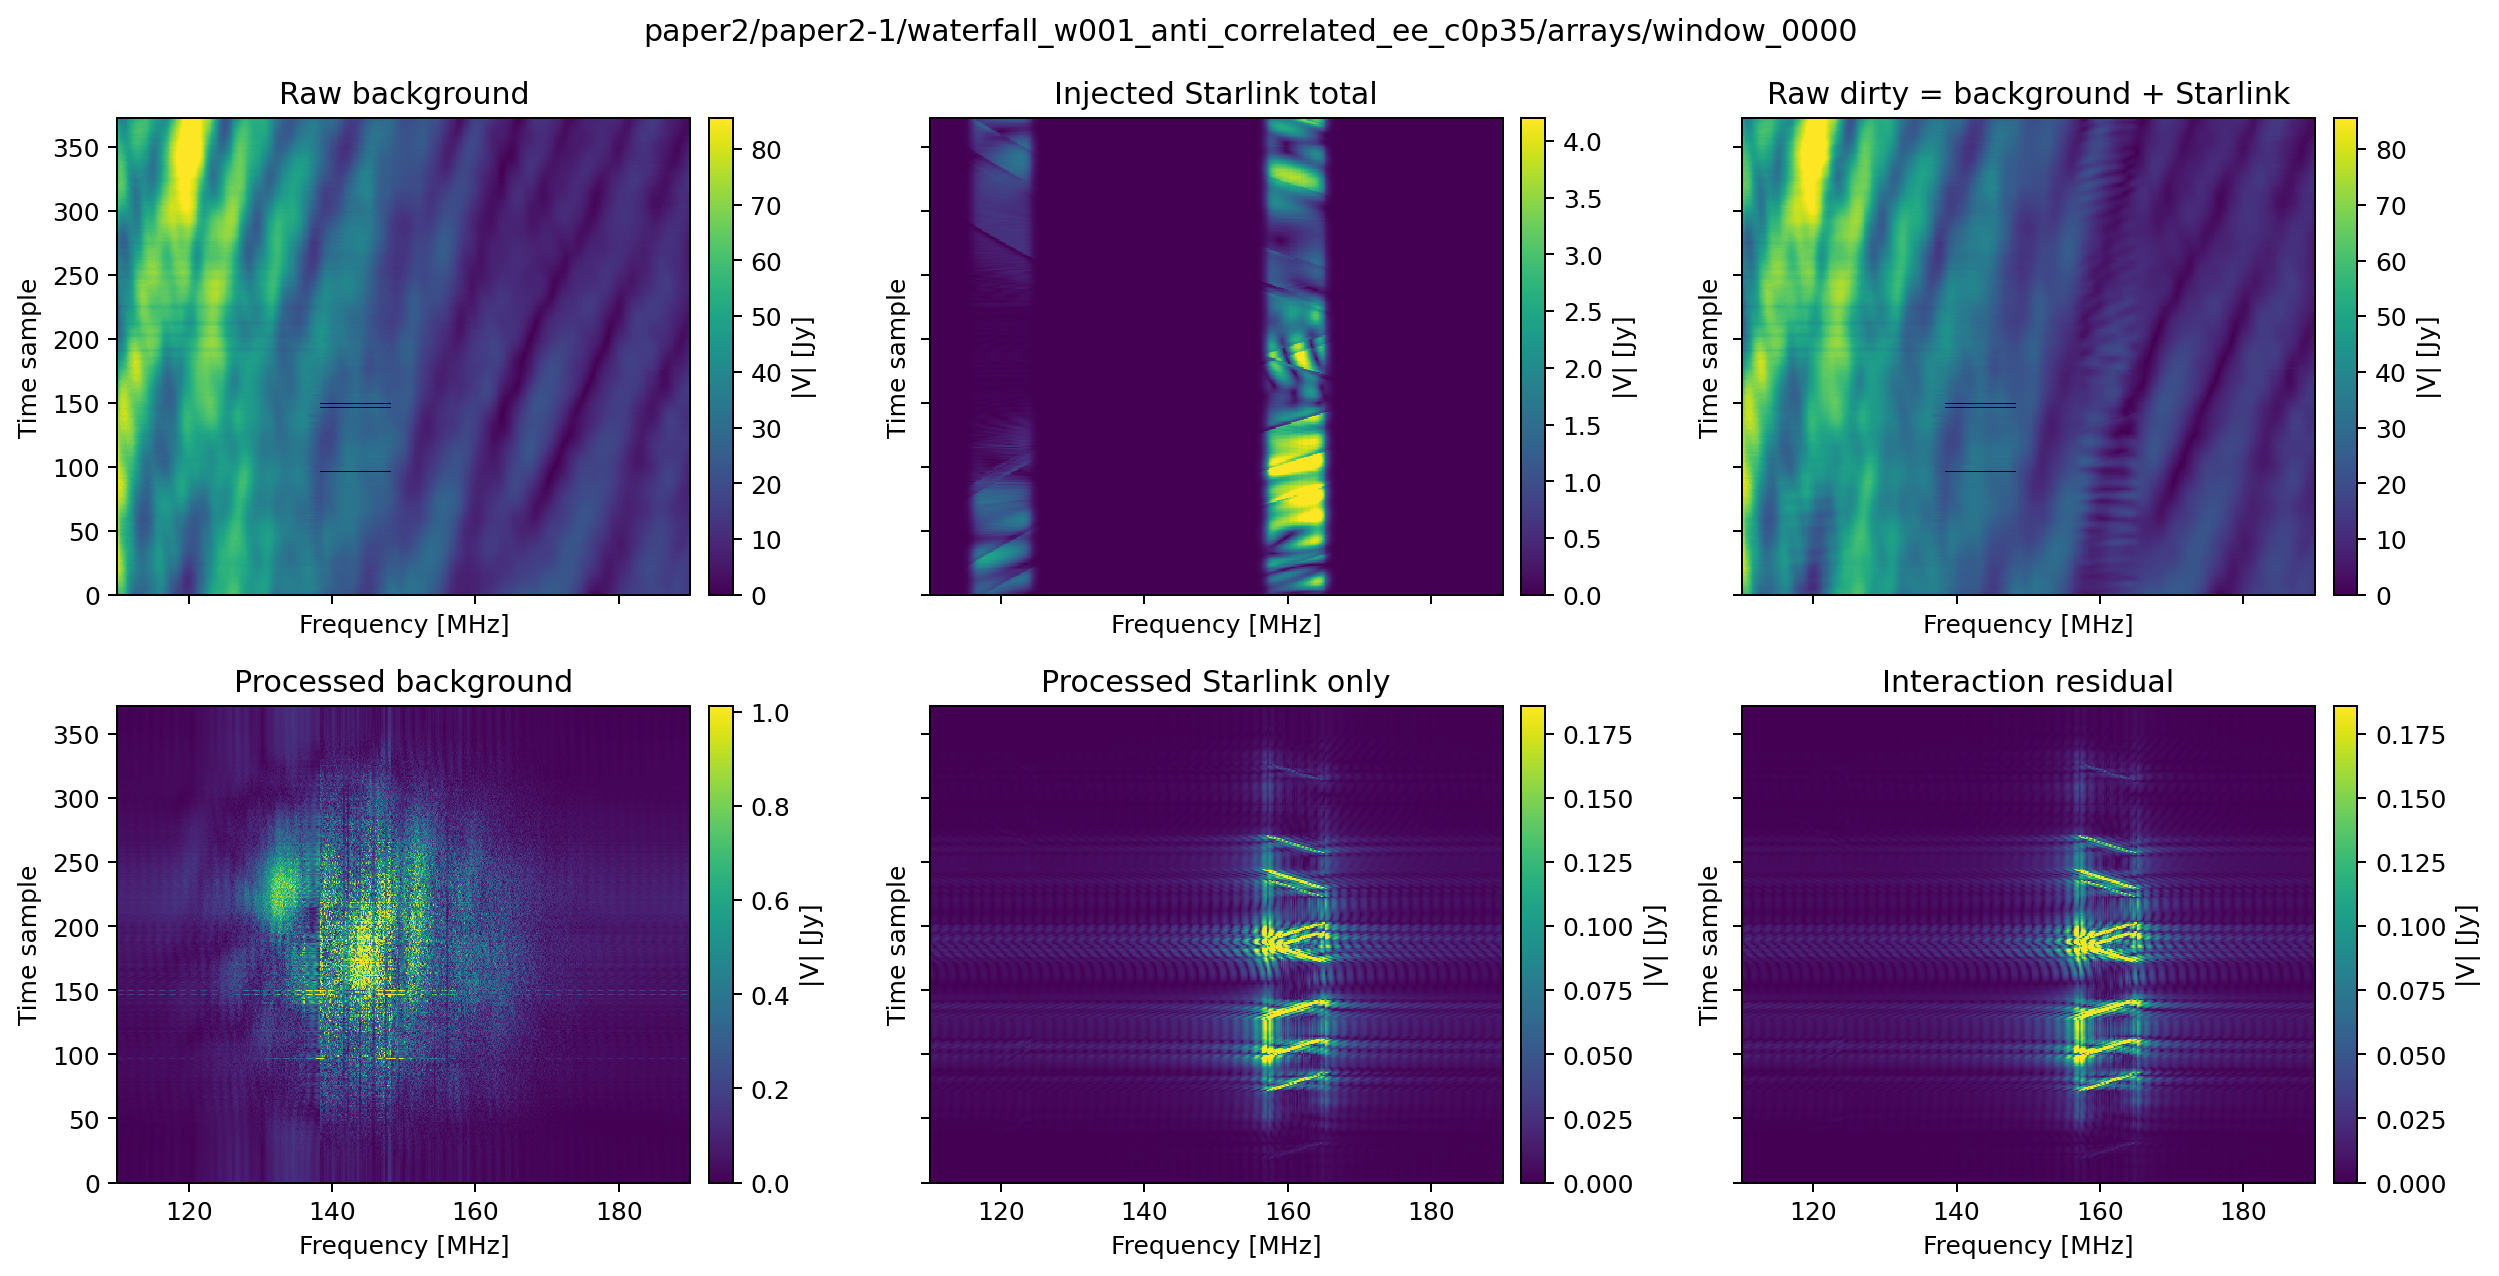
\includegraphics[width=\linewidth]{waterfall_w001_anti_correlated_ee_c0p35/figures/waterfall_raw_processed_6panel_masked.png}
\caption{
대표 w001, EE, anti-correlated contrast 0.35, top-50 emitter run의 raw/processed waterfall.
회색 overlay는 raw background의 invalid samples를 표시한다.
Invalid samples는 rows 96, 146, 149 및 138.35--148.12 MHz에 위치하며, signal로 해석하지 않는다.
}
\label{fig:waterfall}
\end{figure}

Fig.~\ref{fig:waterfall}은 raw background, injected Starlink total, raw dirty, processed background, processed Starlink only, interaction residual을 보여준다.
Injected signal은 raw dirty에서 background에 비해 약하지만, processing 이후 interaction residual에 structured component가 남는다.

이 figure의 해석에서 중요한 점은 두 가지이다.
첫째, raw dirty panel에서 satellite component가 visually dominant하지 않다는 점이다.
이는 본 논문의 클레임과 일치한다.
우리는 strong RFI burst를 주입한 것이 아니라, background 아래에 있는 weak moving emitter contamination이 processing 이후 어떻게 남는지를 본다.
둘째, processed panels에서 residual이 완전히 사라지지 않는다는 점이다.
Delay/fringe processing은 smooth foreground와 일부 stationary structure를 줄이지만, moving emitter의 time-dependent delay/fringe track은 interaction residual로 남을 수 있다.

또한 invalid sample mask가 figure 해석을 안정화한다.
NaN stripe를 흰색으로 방치하면 satellite contamination처럼 오해될 수 있다.
회색 mask overlay는 ``이 pixel은 background product의 invalid sample이며, injected signal이나 residual claim에 사용하지 않는다''는 사실을 명확히 한다.

\subsection{Polarization sensitivity}
\label{sec:pol}

\begin{figure}[t]
\centering
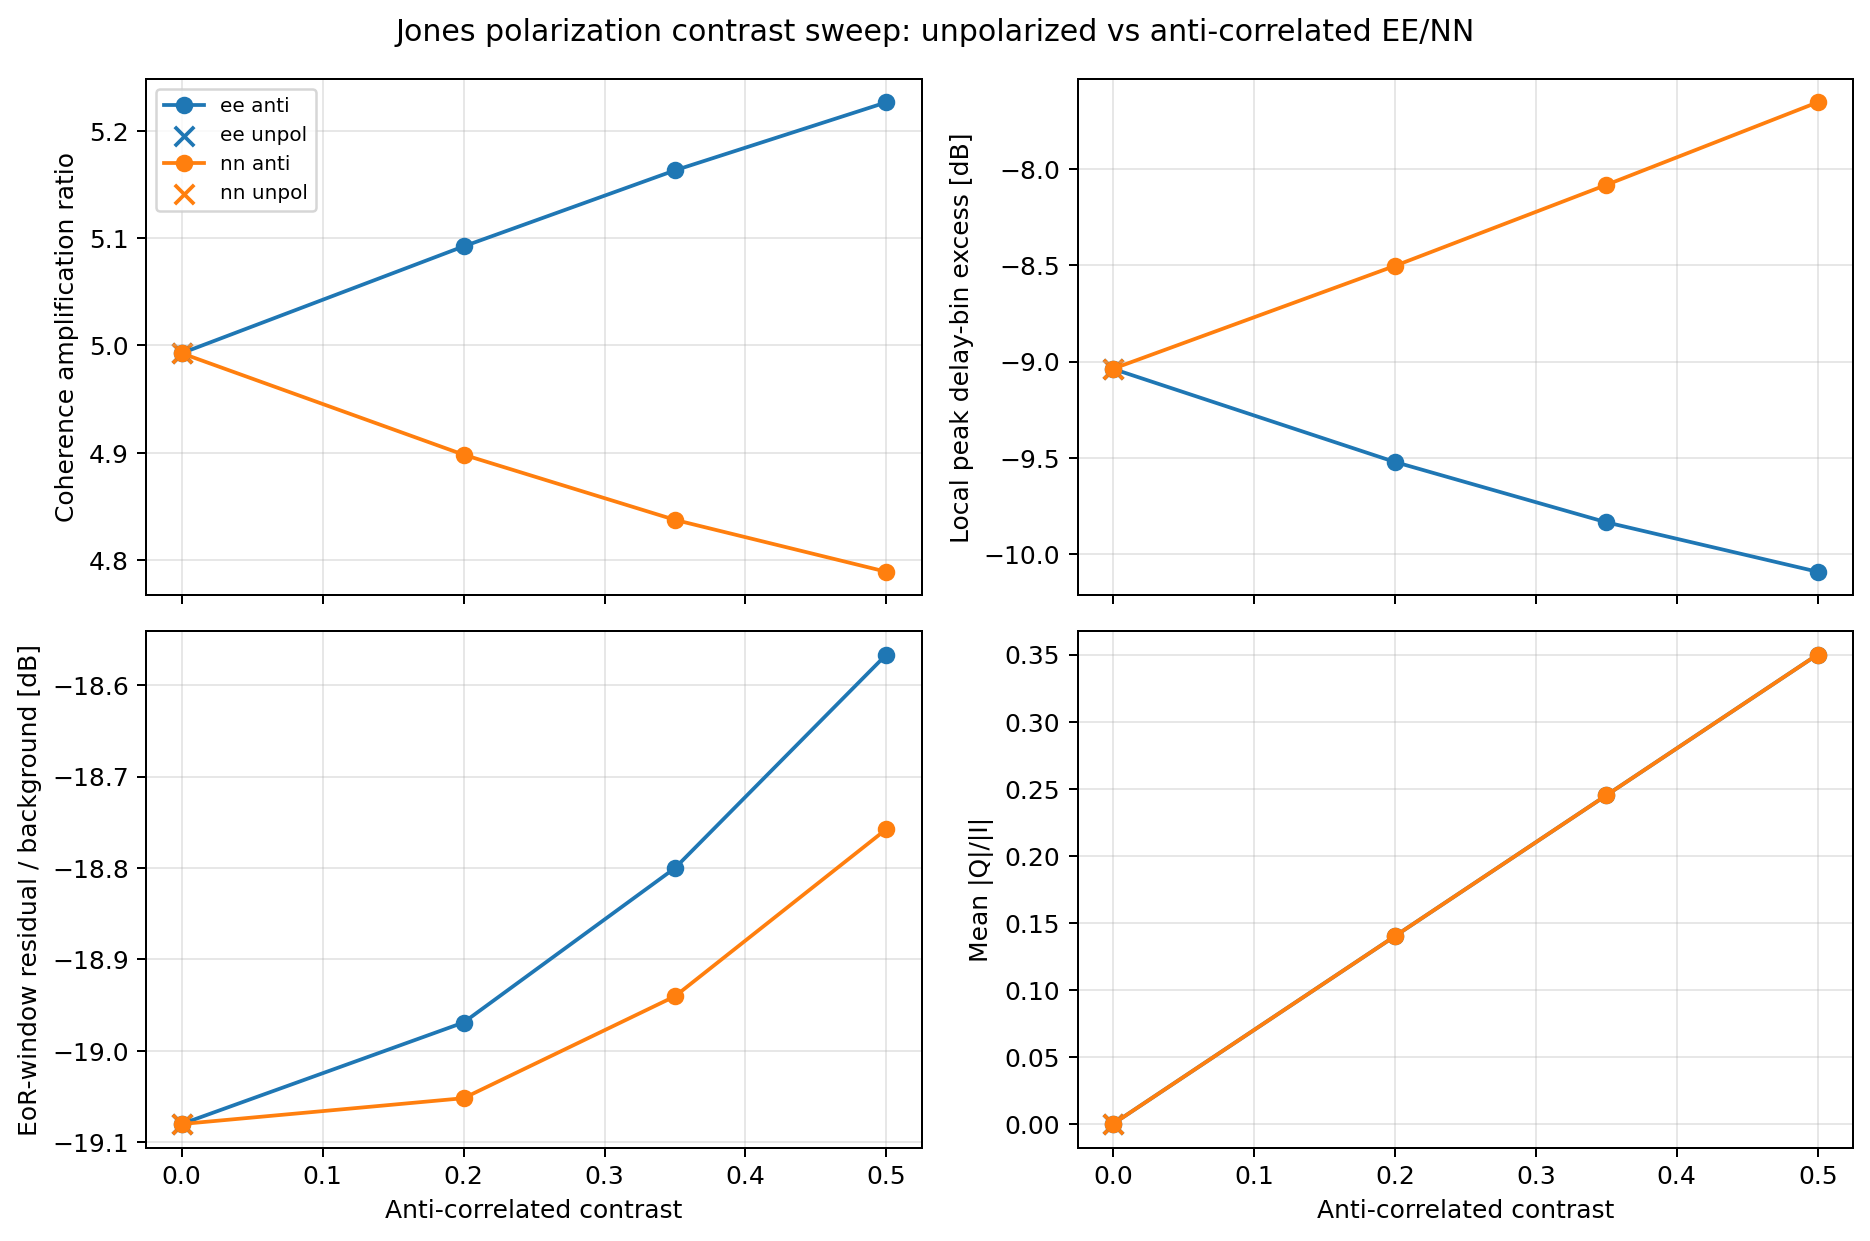
\includegraphics[width=0.9\linewidth]{polarization_contrast_sweep_w001/polarization_contrast_sweep_summary.png}
\caption{
Unpolarized 및 anti-correlated Jones coherency model의 EE/NN contrast sweep.
Anti-correlated model은 parameterized Stokes-Q contrast로 구현하였다.
}
\label{fig:pol-sweep}
\end{figure}

\begin{table}[t]
\centering
\caption{w001 top-50에서 polarization contrast sweep 결과. $Q/I$는 mean absolute Stokes ratio이다.}
\label{tab:pol-sweep}
\begin{tabular}{llrrrr}
\toprule
Pol & Model & Contrast & $|Q|/|I|$ & Amp. [dB] & Local peak [dB]\\
\midrule
EE & unpolarized & --   & 0.000 & 6.98 & -9.04\\
EE & anti-corr.  & 0.20 & 0.140 & 7.07 & -9.52\\
EE & anti-corr.  & 0.35 & 0.245 & 7.13 & -9.83\\
EE & anti-corr.  & 0.50 & 0.350 & 7.18 & -10.09\\
NN & unpolarized & --   & 0.000 & 6.98 & -9.04\\
NN & anti-corr.  & 0.20 & 0.140 & 6.90 & -8.50\\
NN & anti-corr.  & 0.35 & 0.245 & 6.85 & -8.08\\
NN & anti-corr.  & 0.50 & 0.350 & 6.80 & -7.65\\
\bottomrule
\end{tabular}
\end{table}

Anti-correlated model이 적용되면 EE와 NN residual metrics가 서로 달라진다.
EE에서는 contrast가 증가할수록 coherent-like amplification이 약간 증가하고, NN에서는 감소한다.
이는 parameterized Stokes-Q contrast가 pipeline metric에 실제로 영향을 준다는 것을 보여준다.
동시에 모든 tested contrast에서 phase-randomized null 초과 여부는 유지되므로, coherent-like amplification claim은 특정 polarization contrast 하나에만 의존하지 않는다.

이 결과는 두 방향으로 해석된다.
첫째, Jones coherency module은 단순 decoration이 아니다.
Anti-correlated contrast가 EE/NN metric을 실제로 바꾸므로, polarization 가정은 residual amplitude와 local metric에 영향을 준다.
둘째, 본 논문의 main mechanism은 polarization model 하나에 의해 artificially 생성된 것이 아니다.
Unpolarized case와 anti-correlated case 모두에서 observed amplification은 null p95보다 크다.
따라서 polarization uncertainty는 amplitude/detail uncertainty로 남지만, delay-overlap-driven coherent-like amplification 자체를 제거하지 않는다.

다만 현재 table에서 XX/YY power ratio는 일부 과거 run에서 저장되지 않았다.
최종본에서는 최신 code로 A sweep을 재실행하여 $P_{\rm XX}/P_{\rm YY}$를 table에 채운다.
\todo{A sweep 재실행 후 XX/YY power ratio table 업데이트}

\subsection{Phase-randomized null}

\begin{figure}[t]
\centering
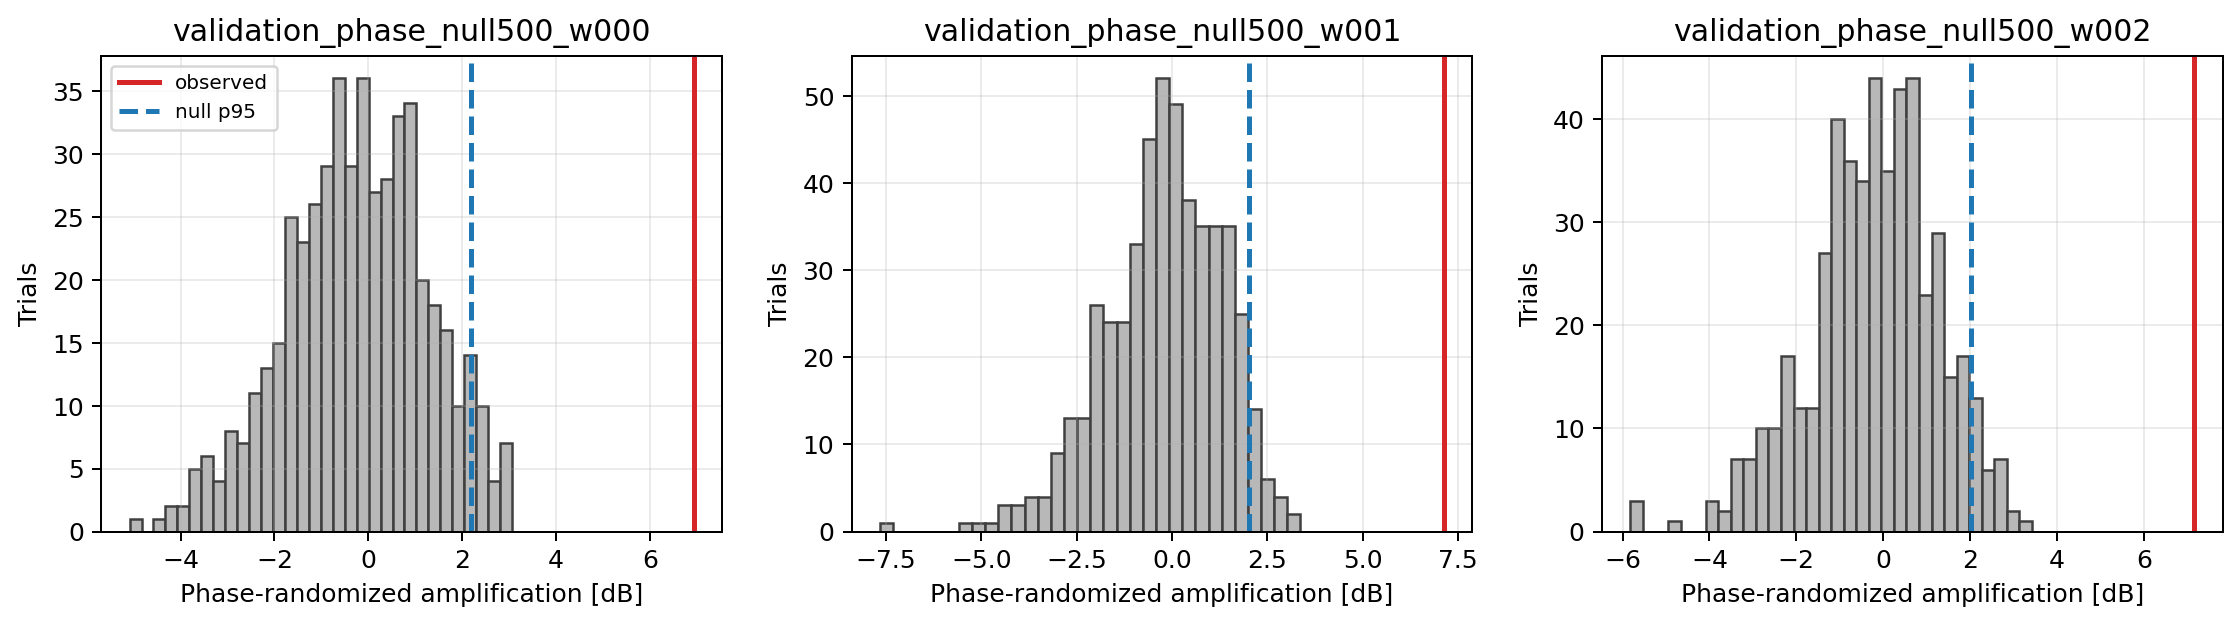
\includegraphics[width=\linewidth]{validation_figures_phase_null500_w000_w002/fig_phase_randomized_null_histograms.png}
\caption{
w000--w002의 phase-randomized null distribution.
각 panel은 500 trials를 포함하며, red vertical line은 observed amplification, blue dashed line은 null p95이다.
}
\label{fig:null-hist}
\end{figure}

\begin{table}[t]
\centering
\caption{Phase-randomized null N=500 검증. 모든 window에서 observed amplification은 null p95를 초과한다.}
\label{tab:null}
\begin{tabular}{lrrrrr}
\toprule
Window & Used & Obs. [dB] & Null p95 [dB] & Obs. $>$ p95 & Local peak [dB]\\
\midrule
w000 & 50 & 6.93 & 2.18 & yes & -23.30\\
w001 & 50 & 7.13 & 2.03 & yes & -9.83\\
w002 & 50 & 7.16 & 2.02 & yes & -4.13\\
\bottomrule
\end{tabular}
\end{table}

Fig.~\ref{fig:null-hist}와 Table~\ref{tab:null}은 observed complex-sum amplification이 random phasor addition alone으로 설명되지 않음을 보여준다.
세 window 모두에서 observed amplification은 phase-randomized null ensemble의 95 percentile을 초과한다.

이 결과의 강점은 null ensemble이 emitter별 amplitude와 delay support를 유지한다는 점이다.
즉 null은 ``같은 밝기와 같은 support를 가진 emitter들이 random phase로 더해졌을 때''의 expectation을 나타낸다.
Observed result가 이 null보다 크다는 것은, 단순히 bright emitters가 많아서 생긴 power 증가가 아니라, 실제 deterministic phase/delay relation이 delay-excess metric을 더 크게 만든다는 뜻이다.

w000은 local peak residual이 약하지만 observed amplification은 여전히 null p95를 넘는다.
w001과 w002는 local residual budget이 더 커지고, 특히 w002는 local peak delay-bin excess가 -4.13 dB까지 올라온다.
이는 window별 geometry와 emitter crowding이 residual severity를 조절함을 시사한다.

\subsection{Top-N sensitivity}
\label{sec:topn}

\begin{figure}[t]
\centering
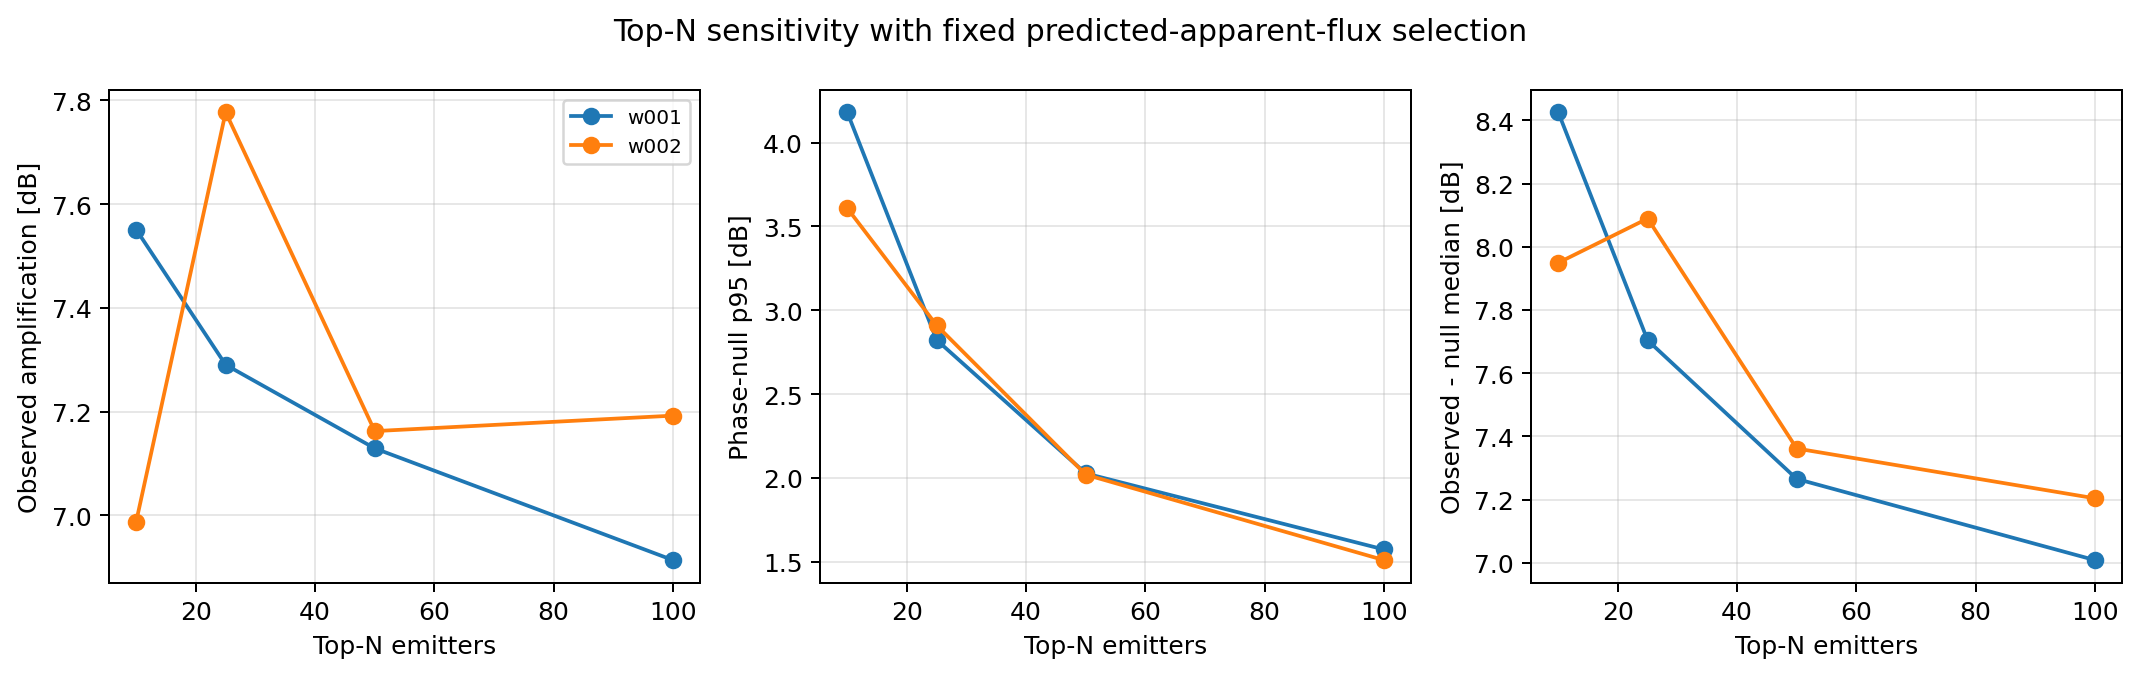
\includegraphics[width=\linewidth]{topn_sensitivity_w001_w002/fig_topn_sensitivity.png}
\caption{
w001 및 w002의 top-N sensitivity.
Emitter subset은 predicted peak apparent flux 기준으로 선택하였다.
}
\label{fig:topn}
\end{figure}

\begin{table}[t]
\centering
\caption{Top-N sensitivity. top-50 선택이 임의적 artifact가 아님을 확인하기 위한 검증이다.}
\label{tab:topn}
\begin{tabular}{llrrrrr}
\toprule
Window & Top-N & Used & Obs. [dB] & Null p95 [dB] & Obs-null med. [dB] & Local peak [dB]\\
\midrule
w001 & 10  & 10  & 7.55 & 4.18 & 8.43 & -19.77\\
w001 & 25  & 25  & 7.29 & 2.82 & 7.70 & -15.94\\
w001 & 50  & 50  & 7.13 & 2.03 & 7.27 & -9.83\\
w001 & 100 & 100 & 6.91 & 1.57 & 7.01 & -6.39\\
w002 & 10  & 10  & 6.99 & 3.61 & 7.95 & -11.56\\
w002 & 25  & 25  & 7.78 & 2.91 & 8.09 & -6.73\\
w002 & 50  & 50  & 7.16 & 2.02 & 7.36 & -4.13\\
w002 & 100 & 100 & 7.19 & 1.51 & 7.20 & -1.49\\
\bottomrule
\end{tabular}
\end{table}

Top-N sensitivity는 두 가지를 보여준다.
첫째, observed-minus-null median margin은 모든 top-N 조건에서 크게 양수이다.
둘째, $N$이 커질수록 local peak delay-bin excess는 background level에 더 가까워진다.
즉 top-50 결과는 특정 arbitrary cap에서만 생긴 현상이 아니며, crowded bright-emitter subset이 residual budget을 증가시킨다는 해석과 일치한다.

w001에서는 observed amplification dB가 top-N이 커질수록 약간 감소하지만, null p95도 함께 감소하고 observed-minus-null median margin은 계속 크게 양수이다.
동시에 interaction vs background와 local peak metric은 N이 커질수록 background level에 가까워진다.
이는 많은 emitter를 포함할수록 total residual budget은 커지지만, coherent-like amplification ratio 자체는 strongest subset에서 이미 saturation될 수 있음을 의미한다.

w002에서는 top-25가 가장 큰 observed amplification을 보이며, top-50/top-100에서도 null 대비 margin은 유지된다.
따라서 top-N 결과는 단순 monotonic increase 하나로 요약되기보다는, ``strongest delay-overlapping subset이 amplification ratio를 지배하고, 더 많은 emitter는 local residual budget을 증가시킨다''로 해석하는 것이 더 정확하다.
이 해석은 crowded constellation risk를 주장하면서도 top-50 cap의 임의성을 정직하게 다룬다.

\subsection{Pairwise same-delay-bin overlap}

\begin{figure}[t]
\centering
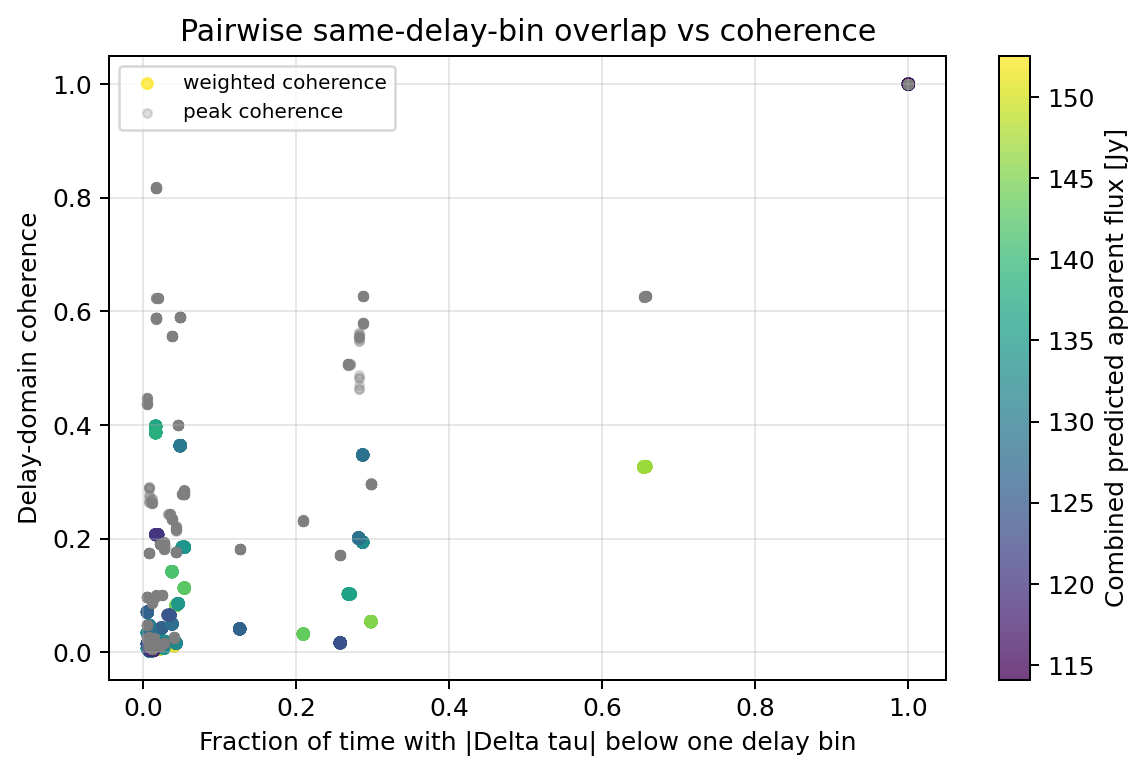
\includegraphics[width=0.85\linewidth]{validation_phase_null500_w001/figures/fig05_pairwise_delay_separation_vs_coherence.png}
\caption{
w001 top-50의 pairwise same-delay-bin overlap vs weighted delay-domain coherence.
x-axis는 $\mathrm{fraction\_time}(|\Delta\tau_{ij}|<\Delta\tau_{\rm bin})$이며, color는 combined predicted apparent flux를 나타낸다.
}
\label{fig:pairwise}
\end{figure}

Pairwise coherence outlier는 단순히 instantaneous minimum $\Delta\tau$가 작다는 사실만으로는 설명하기 어렵다.
Fig.~\ref{fig:pairwise}는 high pairwise coherence가 같은 delay bin에 상당 시간 머무는 emitter pairs에 집중됨을 보여준다.
이는 다중 emitter coherent-like amplification의 물리적 설명을 제공한다.

이 figure는 본 논문의 mechanism figure이다.
Null histogram이 ``random phase만으로는 설명되지 않는다''를 보여준다면, pairwise overlap figure는 ``무엇이 설명하는가''를 보여준다.
Delay tracks가 같은 bin에 오래 머물면 weighted delay-domain coherence가 커지고, 이러한 pair들이 multi-emitter sum에서 coherent-like excess를 만든다.

최종본에서는 figure caption에 delay-bin width, frequency bandwidth로부터 유도된 delay resolution, color/size encoding을 명시해야 한다.
\todo{delay bin width numerical value와 colorbar range를 caption에 추가}

\subsection{Local residual budget}

\begin{figure}[t]
\centering
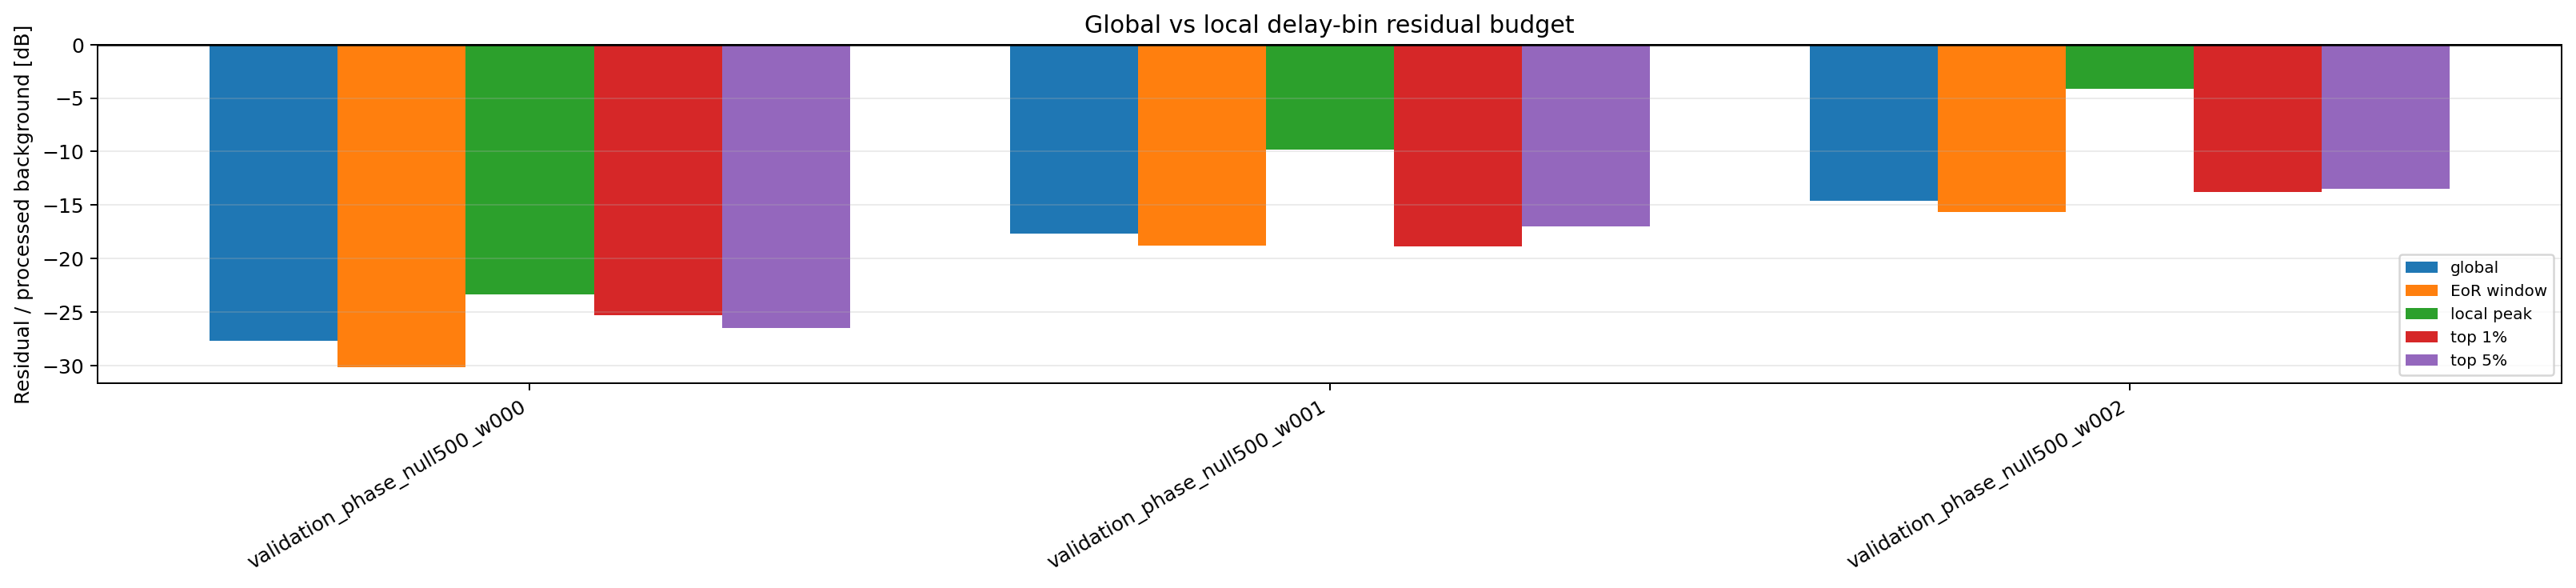
\includegraphics[width=0.9\linewidth]{validation_figures_phase_null500_w000_w002/fig_local_residual_budget_bars.png}
\caption{
Global processed-background ratio와 local/EoR-window delay-bin residual metric 비교.
Residual은 total processed background power를 지배하지 않지만, local delay-bin 기준에서는 global metric보다 background level에 더 가까워진다.
}
\label{fig:local-budget}
\end{figure}

\begin{table}[t]
\centering
\caption{Local residual budget metric.}
\label{tab:local}
\begin{tabular}{lrrrr}
\toprule
Window & Global [dB] & Local peak [dB] & Top 1\% [dB] & Top 5\% [dB]\\
\midrule
w000 & -27.69 & -23.30 & -25.30 & -26.45\\
w001 & -17.69 & -9.83  & -18.84 & -17.01\\
w002 & -14.61 & -4.13  & -13.80 & -13.50\\
\bottomrule
\end{tabular}
\end{table}

전체 processed background 대비 residual은 subdominant이다.
그러나 local peak delay-bin excess는 global metric보다 훨씬 덜 음수이며, 특히 w002에서는 -4.13 dB까지 접근한다.
따라서 ``background 전체를 이기는가''가 아니라, 분석상 중요한 delay-bin residual budget을 얼마나 왜곡하는가가 핵심이다.

이 결과는 본 논문 claim의 중요한 nuance를 만든다.
Starlink-like residual은 전체 processed visibility power를 압도하지 않는다.
따라서 단순 total-power RFI metric으로는 ``문제가 작다''고 결론낼 수 있다.
하지만 delay-spectrum analysis에서는 특정 delay bins가 cosmological inference에 더 중요하다.
그 bins에서 residual이 background level에 가까워지면, total power가 작더라도 inference bias 또는 excess variance risk가 생긴다.

이 점은 PDF 초안의 ``보이지 않는 부재가 아니라 distorted/misleading residual'' 논리와 연결된다.
즉 contamination은 반드시 눈에 띄는 bright artifact일 필요가 없다.
Processing 이후 특정 analysis subspace에 남는 structured residual이면 충분히 problematic하다.

\section{논의}

\subsection{왜 raw visibility가 아니라 interaction residual인가}

Raw visibility에서 satellite injection이 background보다 약하다는 사실은 contamination risk가 없다는 뜻이 아니다.
HERA-like analysis는 raw visibility를 직접 해석하지 않고, delay/fringe filtering, averaging, power-spectrum-like metric을 거친다.
따라서 relevant observable은 raw satellite amplitude가 아니라 processing 이후 residual이다.

Interaction residual은 nonlinearity가 없는 linear processing에서도 의미가 있다.
왜냐하면 ${\cal P}(\vis_{\rm bg}+\vis_{\rm sat})-{\cal P}(\vis_{\rm bg})$는 processed satellite-only component와 같아 보일 수 있지만, 실제 implementation에서는 weights, invalid samples, finite transforms, filtering choices, product-level metric이 결합된다.
또한 논문 claim은 visibility 자체보다 delay-excess metric, local bin excess, subspace overlap에 관한 것이다.
따라서 interaction residual을 명시적으로 저장하고 figure로 보여주는 것이 가장 안전하다.

\subsection{Coherent-like라는 표현의 의미}

본 논문은 ``coherent-like amplification''이라는 표현을 사용한다.
이는 satellite들이 서로 phase-locked되어 있다는 뜻이 아니다.
오히려 같은 delay bin에 머무는 moving emitters가 deterministic phase/delay relation을 가지며, 이 관계가 delay-domain metric에서 random phase null보다 큰 excess를 만든다는 뜻이다.

따라서 claim은 operational하다.
우리는 observed complex sum을 만들고, 같은 amplitudes와 supports를 가진 phase-randomized ensemble을 만든다.
Observed가 null p95를 넘으면, random phasor addition alone으로 설명되지 않는 coherent-like excess라고 부른다.
이 정의는 물리적 synchronization을 요구하지 않으므로 LEO constellation 상황에 더 적합하다.

\subsection{Top-N cap의 의미}

Top-N cap은 두 가지 이유로 필요하다.
첫째, 계산량을 제한한다.
둘째, main risk가 bright subset에 의해 지배되는지 확인할 수 있다.
그러나 cap이 임의적이면 result shopping처럼 보일 수 있다.
따라서 cap selection score를 predicted peak apparent flux로 고정하고, top-N sensitivity를 수행했다.

결과적으로 top-50은 대표 선택일 뿐, 유일하게 현상이 나타나는 선택이 아니다.
top-10, top-25, top-50, top-100 모두 observed-minus-null median margin이 양수이다.
다만 local residual budget은 N에 따라 커지며, amplification ratio는 strongest subset에서 saturation 또는 non-monotonic behavior를 보인다.
이는 ``많을수록 무조건 ratio가 커진다''보다 더 물리적인 결과이다.

\subsection{Polarization uncertainty}

Polarization sensitivity는 본 논문의 불확실성 중 하나를 정직하게 드러낸다.
Anti-correlated contrast가 EE와 NN metric을 다르게 만들기 때문에, 실제 satellite polarization state는 residual severity에 영향을 줄 수 있다.
그러나 unpolarized case에서도 null exceedance가 유지되므로, coherent-like amplification mechanism은 polarization model 하나에 의존하지 않는다.

최종적인 real-data interpretation에서는 simultaneous EE/NN/EN/NE measurement가 필요하다.
특히 D-terms와 Faraday rotation이 존재하면 Stokes leakage가 생길 수 있다.
본 논문의 diagonal Jones model은 첫 번째 sensitivity step이며, full-polarization propagation은 후속 연구로 남긴다.

\subsection{Invalid samples와 figure ethics}

NaN stripe를 그대로 흰색으로 표시하면 figure가 misleading해진다.
본 연구에서는 raw background의 invalid region을 확인하고 mask overlay로 표시하였다.
이것은 작은 plotting detail이 아니라, contamination paper에서 매우 중요한 ethics issue이다.
실제 signal이 아닌 missing data를 dramatic residual처럼 보이게 하면 논문 claim이 약해진다.
따라서 모든 representative waterfall은 invalid mask와 함께 제시되어야 한다.

\section{아직 닫히지 않은 검증}
\label{sec:future}

다음 항목은 본문 claim을 더 강하게 만들기 위해 필요하지만, 현재 초안에서는 아직 비워둔다.

\subsection{Subspace non-identifiability}

\todo{
processed background, interaction residual, EoR-like proxy에 대해 SVD subspace overlap을 계산한다.
$k=1,2,3,5,10$에 대해
$\|U_a^\dagger U_b\|_F/\sqrt{k}$ 및 principal angle min/median을 저장한다.
Heatmap figure를 추가한다.
}

이 검증은 본 논문의 다음 단계에서 가장 중요하다.
현재 A--E 실험은 residual이 존재하고, null을 초과하며, local delay-bin budget을 증가시킨다는 것을 보여준다.
하지만 PDF의 더 큰 철학인 ``subspace non-identifiability''를 닫으려면, residual이 foreground/EoR-like low-rank subspace와 얼마나 겹치는지 수치로 보여줘야 한다.

구체적으로 다음 행렬을 비교한다.
\[
  X_{\rm bg}={\cal P}(\vis_{\rm bg}),\quad
  X_{\rm sat}=\vis_{\rm int},\quad
  X_{\rm eor}=\todo{EoR-like proxy}.
\]
각 행렬에 대해 SVD를 수행하고,
\[
  {\cal O}_{ab}(k)
  =
  \frac{\|U_a[:,1:k]^\dagger U_b[:,1:k]\|_F}{\sqrt{k}}
\]
를 계산한다.
$k=1,2,3,5,10$을 sweep하고, principal angle min/median을 함께 저장한다.
이 결과가 나오면 satellite residual이 단순 narrowband RFI처럼 완전히 orthogonal한 것이 아니라, 분석 subspace와 겹칠 수 있음을 보여줄 수 있다.

\subsection{Window expansion}

\todo{
w000--w010으로 확대한다.
동일 조건: mid-alt gate, top-50 predicted apparent flux, EE, anti-correlated contrast 0.35, phase-null N=500 또는 N=200.
대표 figure는 w001/w002를 쓰고, 나머지는 appendix table로 둔다.
}

현재 main validation은 w000--w002 세 window에 기반한다.
이는 mechanism demonstration으로는 충분하지만, 일반성 주장에는 부족하다.
최소 w000--w010까지 확장하면 window-to-window variation을 보여줄 수 있다.
다만 이 확장은 새로운 아이디어 실험이 아니라 robustness table이다.
따라서 figure를 무리하게 늘리기보다, summary table과 appendix histogram grid로 처리하는 것이 좋다.

\subsection{Altitude 및 baseline sensitivity}

\todo{
선택 실험.
Altitude gate는 low 10--35, mid 35--65, high 65--85 degree로 비교한다.
Baseline sensitivity는 short/current/long baseline이 가능할 때만 수행한다.
}

Altitude sensitivity는 near-zenith compression 문제와 연결된다.
Low-altitude pass는 beam/range가 약하지만 duration이 길 수 있고, high-altitude pass는 강하지만 support가 압축될 수 있다.
따라서 representative main-text example은 mid-altitude가 적합하며, high-altitude/zenith case는 rejected sanity example로 appendix에 둘 수 있다.

Baseline sensitivity는 현재 single-baseline limitation을 완화한다.
가능하다면 short baseline과 longer baseline을 하나씩 추가하여 delay-bin width, horizon delay, fringe-rate response가 metric에 미치는 영향을 확인한다.
그러나 baseline sensitivity는 본문 core claim보다 robustness check에 가깝다.

\section{한계}

본 연구는 다음 한계를 가진다.

\begin{enumerate}
  \item Starlink proprietary waveform을 재현하지 않는다.
  \item Source coherency $C_{\rm src}$는 literature-motivated parameterization이며, 실제 full-Stokes measurement가 아니다.
  \item D-terms, mutual coupling, Faraday rotation, Stokes U/V는 포함하지 않는다.
  \item 현재 main validation은 단일 baseline 및 w000--w002 window에 국한되어 있다. \todo{w000--w010 확대 후 업데이트}
  \item Background crop에는 NaN invalid samples가 존재하며, figure에서는 mask overlay로 처리하였다.
  \item Top-N cap은 computationally motivated selection이며, 본문에서는 predicted apparent flux 기준과 top-N sensitivity를 함께 보고한다.
\end{enumerate}

\section{결론}

본 논문은 약한 Starlink-like UEMR이 raw visibility에서는 background에 묻힐 수 있으나, HERA-like delay/fringe processing 이후 structured interaction residual로 남을 수 있음을 controlled injection으로 보였다.
또한 다중 emitter 조건에서 observed delay-domain coherent-like amplification이 phase-randomized null ensemble의 95 percentile을 초과함을 w000--w002 세 window에서 확인하였다.

Polarization sensitivity 실험은 Bassa-style XX/YY anti-correlation을 parameterized Stokes-Q contrast로 넣었을 때 EE와 NN residual metric이 달라짐을 보여준다.
그러나 coherent-like amplification claim은 특정 polarization contrast 하나에만 의존하지 않았다.
Top-N sensitivity는 top-50 cap이 arbitrary artifact가 아님을 보였고, local residual budget 분석은 global processed-background ratio만으로는 contamination risk를 과소평가할 수 있음을 보였다.

따라서 본 연구의 결론은 다음과 같다.
\begin{quote}
Starlink-like moving-emitter contamination은 total background power를 지배하지 않더라도, HERA-like delay/fringe processing 이후 분석상 중요한 delay-domain residual budget을 구조적으로 증가시킬 수 있으며, 다중 emitter delay overlap 조건에서는 random phase null을 초과하는 coherent-like amplification을 만들 수 있다.
\end{quote}

\appendix

\section{Appendix A: 실행 산출물과 파일 구조}

본문의 주요 결과는 다음 디렉터리에 저장되어 있다.
\begin{itemize}
  \item Polarization sensitivity: \texttt{polarization\_contrast\_sweep\_w001/}
  \item Phase null validation: \texttt{validation\_figures\_phase\_null500\_w000\_w002/}
  \item Top-N sensitivity: \texttt{topn\_sensitivity\_w001\_w002/}
  \item Representative waterfall: \texttt{waterfall\_w001\_anti\_correlated\_ee\_c0p35/}
\end{itemize}

각 output directory에는 \texttt{tables/}, \texttt{figures/}, \texttt{reports/}가 포함된다.
Table과 figure는 가능한 한 code-generated output을 그대로 참조하였다.
이 방식은 수동 transcription error를 줄인다.

\section{Appendix B: 대표 명령어}

대표 phase-null validation run은 다음 형식이다.
\begin{verbatim}
python run_nearfield_starlink_multiwindow_v4.py \
  --config nearfield_starlink_multiwindow_config.yaml \
  --background background_0_5_w001_1h.npz \
  --output-dir validation_phase_null500_w001 \
  --start-window 0 --max-windows 1 \
  --max-sats-per-window 50 \
  --max-scan-satellites 5000 \
  --peak-alt-min-deg 35 --peak-alt-max-deg 70 \
  --cap-selection-method predicted_peak_apparent_flux \
  --pol ee \
  --polarization-mode jones_anti_correlated \
  --polarization-contrast 0.35 \
  --phase-null-trials 500
\end{verbatim}

Top-N sensitivity는 \texttt{run\_topn\_sensitivity\_wsl.ps1}로 실행하였다.
Polarization contrast sweep은 \texttt{run\_polarization\_contrast\_sweep\_wsl.ps1}로 실행하였다.

\section{Appendix C: Metric column dictionary}

\begin{description}
  \item[\texttt{coherence\_amplification\_db}]
  $10\log_{10} R_{\rm obs}$.
  \item[\texttt{phase\_randomized\_null\_ratio\_p95}]
  Phase-randomized null ratio의 95 percentile.
  \item[\texttt{observed\_minus\_phase\_null\_median\_db}]
  Observed amplification과 null median의 dB 차이.
  \item[\texttt{interaction\_vs\_processed\_background\_db}]
  전체 processed background power 대비 interaction residual power.
  \item[\texttt{local\_peak\_delay\_bin\_excess\_db}]
  EoR/delay-excess region에서 가장 큰 delay-bin residual/background ratio.
  \item[\texttt{top\_1\_percent\_delay\_bin\_excess\_db}]
  residual power 기준 상위 1 percent delay bins에서의 residual/background ratio.
  \item[\texttt{fraction\_time\_delta\_tau\_lt\_bin}]
  Pairwise delay tracks가 같은 delay bin 안에 있는 time fraction.
\end{description}

\section{Appendix D: 현재 TODO 목록}

최종 제출 전 반드시 확인할 항목은 다음과 같다.
\begin{enumerate}
  \item 문헌 서지정보: Di Vruno 2023, Bassa 2024, Fagnoni/PolyBeam, HERA instrument, Hamaker/Smirnov measurement equation.
  \item A sweep 최신 code 재실행 후 XX/YY power ratio table 채우기.
  \item Subspace non-identifiability SVD figure 추가.
  \item w000--w010 window expansion table 추가.
  \item Data/code availability 문구 확정.
  \item Figure caption에 exact delay-bin width, frequency bandwidth, integration time 추가.
\end{enumerate}

\section*{Data and code availability}

\todo{GitHub repository URL, commit hash, raw data availability statement를 추가한다. 기본 raw UVH5는 업로드하지 않는다는 정책을 명시한다.}

\section*{Acknowledgements}

\todo{감사의 글}

\begin{thebibliography}{99}

\bibitem{DiVruno2023}
Di Vruno et al. 2023.
\newblock \todo{정확한 제목, 저널, DOI}

\bibitem{Bassa2024}
Bassa et al. 2024.
\newblock \todo{정확한 제목, 저널, DOI}

\bibitem{Fagnoni2021}
Fagnoni et al. 2021.
\newblock HERA primary beam / PolyBeam reference.
\newblock \todo{정확한 제목, 저널, DOI}

\bibitem{Hamaker1996}
Hamaker, Bregman, and Sault. 1996.
\newblock Measurement equation reference.
\newblock \todo{정확한 서지정보}

\bibitem{Smirnov2011}
Smirnov. 2011.
\newblock Radio interferometric measurement equation reference.
\newblock \todo{정확한 서지정보}

\bibitem{HERA}
HERA Collaboration.
\newblock \todo{HERA instrument/pipeline citation}

\end{thebibliography}

\end{document}
